\chapter{Additional Fits}
\label{app:AddFits}
%
%
This appendix contains post-fit signal region plots for alternative fitting methods.  Section \ref{sec:addfitmu} contains the results for simultaneously fitting both regions with the $m_{q\gamma}$ distribution and post-fit distributions for the $\mu$+jets channel and Section \ref{sec:addfitel} contains simultaneous fit restuls for $\gamma$  $p_T$ distributions along with the post-fit distributions for the e+jets channel.

\section{Alternative Fit Method: Both Channels $m_{q\gamma}$}
\label{sec:addfitmu}

\begin{figure}[]
\centering
\subfloat[]{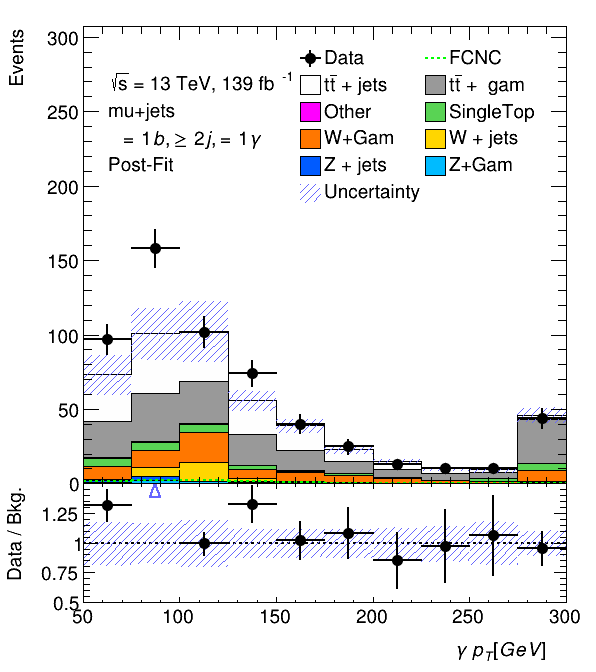
\includegraphics[width=.33\columnwidth]{../ThesisImages/RegionPlots/FinalRegions/Systematics/FCNC_All_mujets/Plots/SRmu_ph_pt_postFit.png}}\hfil
\subfloat[]{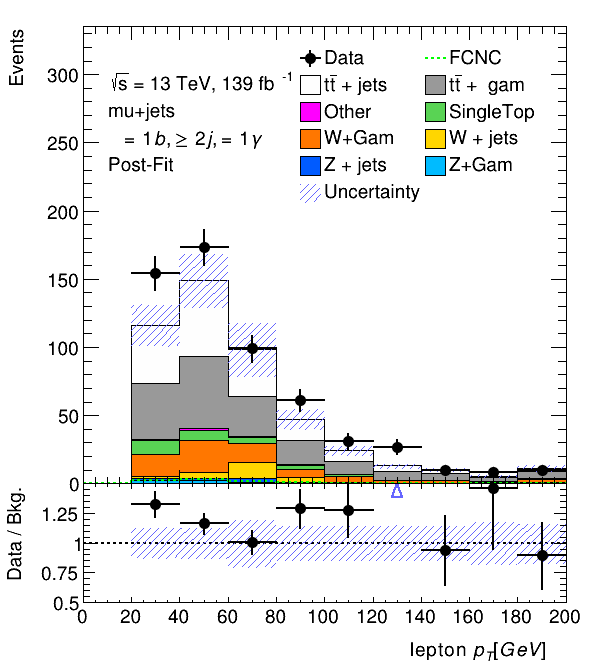
\includegraphics[width=.33\columnwidth]{../ThesisImages/RegionPlots/FinalRegions/Systematics/FCNC_All_mujets/Plots/SRmu_lep_pt_postFit.png}}\hfil  
\subfloat[]{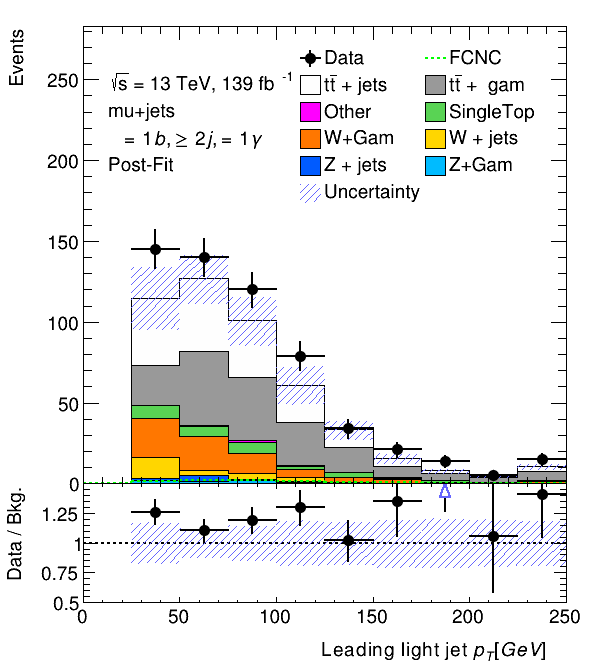
\includegraphics[width=.33\columnwidth]{../ThesisImages/RegionPlots/FinalRegions/Systematics/FCNC_All_mujets/Plots/SRmu_jet0_pt_postFit.png}}
\vspace{-3.mm}
\subfloat[]{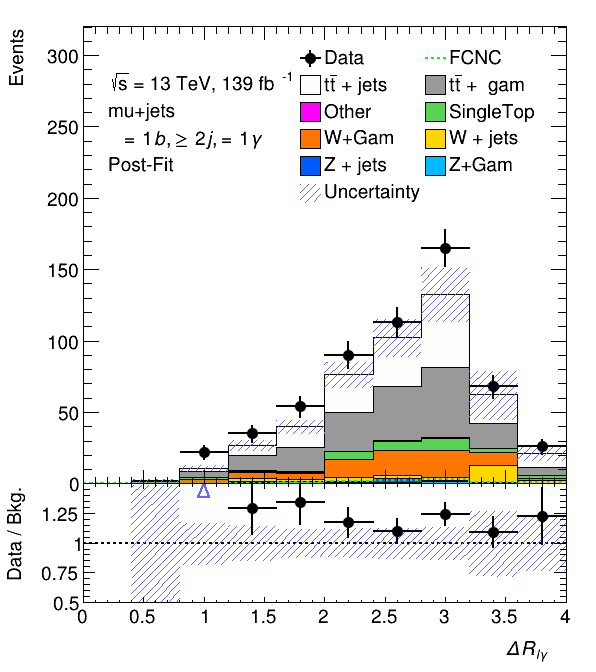
\includegraphics[width=.33\columnwidth]{../ThesisImages/RegionPlots/FinalRegions/Systematics/FCNC_All_mujets/Plots/SRmu_drlph_postFit.png}}\hfil
\subfloat[]{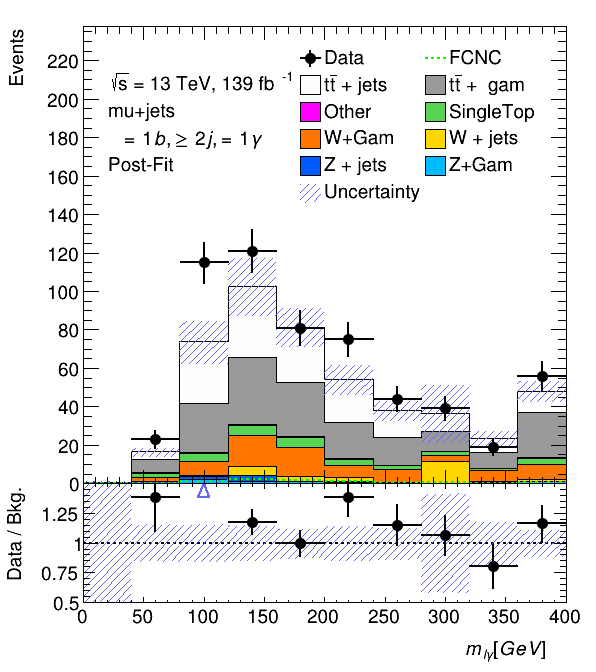
\includegraphics[width=.33\columnwidth]{../ThesisImages/RegionPlots/FinalRegions/Systematics/FCNC_All_mujets/Plots/SRmu_m_lgam_postFit.png}}\hfil 
\subfloat[]{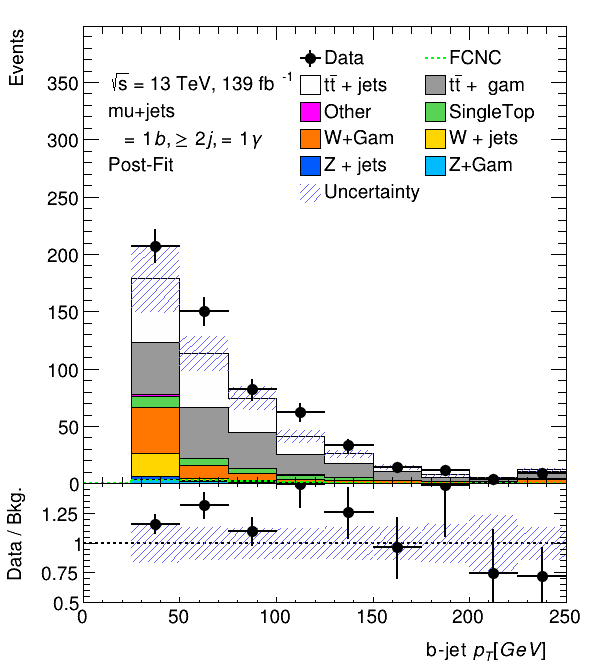
\includegraphics[width=.33\columnwidth]{../ThesisImages/RegionPlots/FinalRegions/Systematics/FCNC_All_mujets/Plots/SRmu_bjet0_pt_postFit.png}}
\caption{Post-fit distributions for Photon $p_T$ (a), lepton $p_T$ (b), leading light jet $p_T$ (c), $\Delta R_{l\gamma}$ (d), $m_{l \gamma}$ (e), and b-jet $p_T$ (f) in the final signal region for the muon channel fitting on  $m_{q\gamma}$. }
\end{figure}


\begin{figure}[]
\centering
\subfloat[]{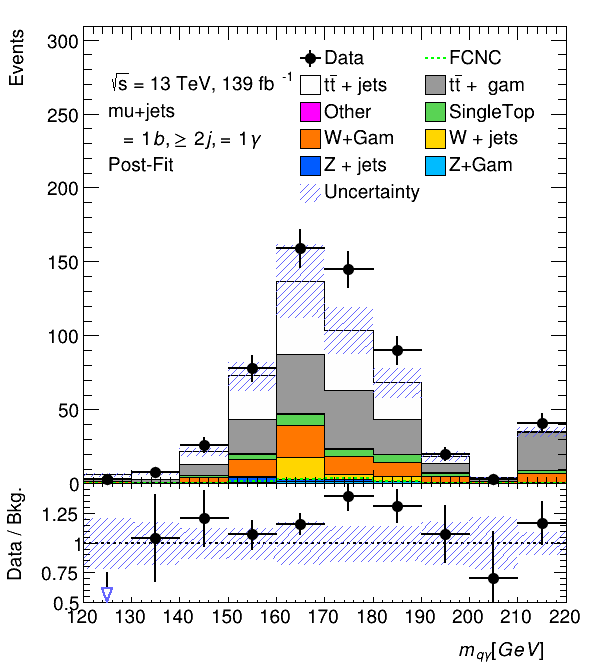
\includegraphics[width=.33\columnwidth]{../ThesisImages/RegionPlots/FinalRegions/Systematics/FCNC_All_mujets/Plots/SRmu_mqph_postFit.png}}\hfil
\subfloat[]{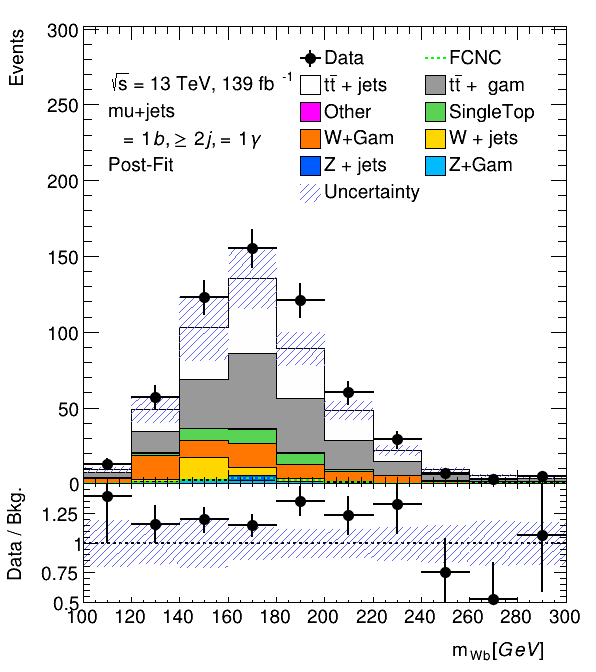
\includegraphics[width=.33\columnwidth]{../ThesisImages/RegionPlots/FinalRegions/Systematics/FCNC_All_mujets/Plots/SRmu_SMtop_postFit.png}}\hfil  
\subfloat[]{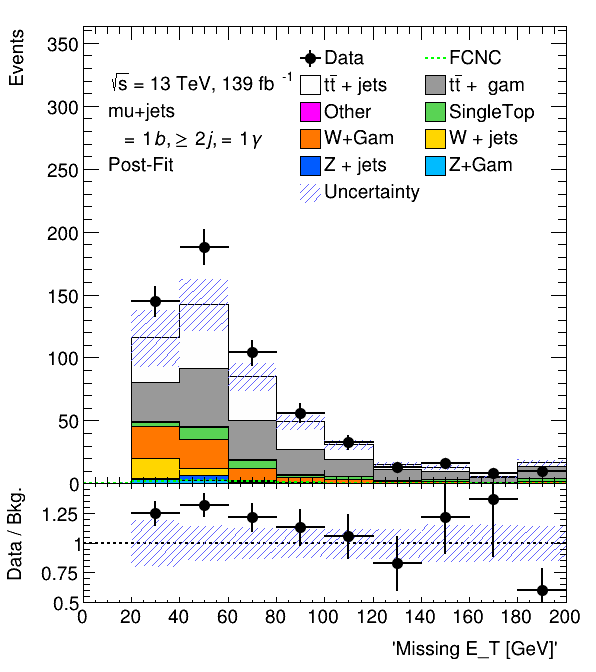
\includegraphics[width=.33\columnwidth]{../ThesisImages/RegionPlots/FinalRegions/Systematics/FCNC_All_mujets/Plots/SRmu_met_postFit.png}}
\vspace{-3.mm}
\subfloat[]{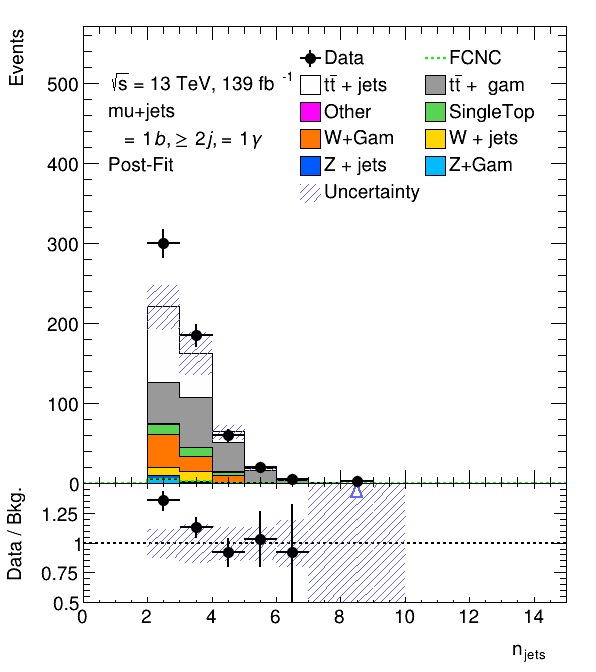
\includegraphics[width=.33\columnwidth]{../ThesisImages/RegionPlots/FinalRegions/Systematics/FCNC_All_mujets/Plots/SRmu_njet_postFit.png}}\hfil
\subfloat[]{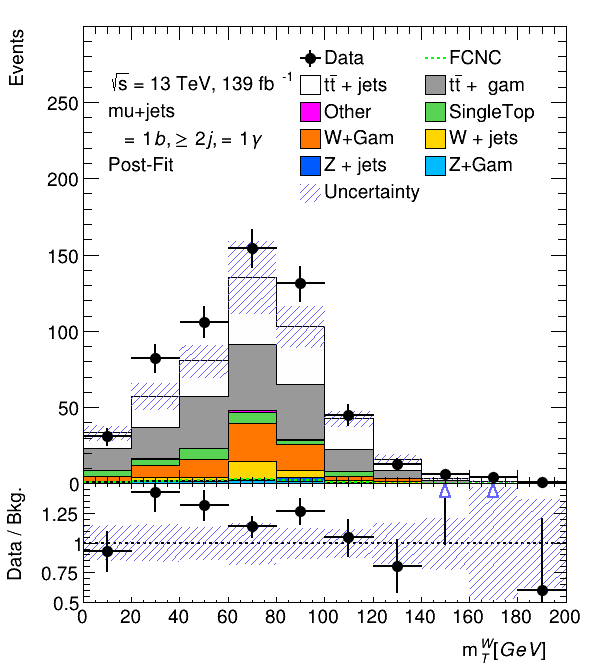
\includegraphics[width=.33\columnwidth]{../ThesisImages/RegionPlots/FinalRegions/Systematics/FCNC_All_mujets/Plots/SRmu_MWT_postFit.png}}\hfil  
\subfloat[]{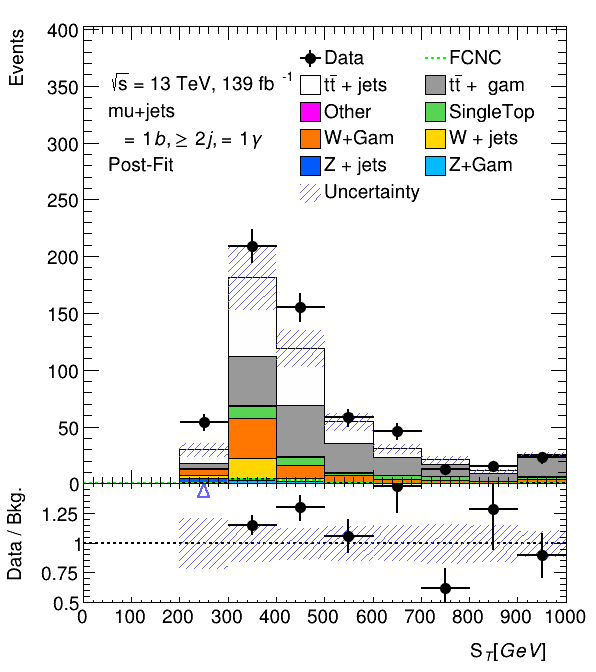
\includegraphics[width=.33\columnwidth]{../ThesisImages/RegionPlots/FinalRegions/Systematics/FCNC_All_mujets/Plots/SRmu_ST_postFit.png}}
\caption{Post-fit distributions for FCNC top candidate mass (a), Standard Model top candidate mass (b), $\slashed{E}_T$ (c), $N_\text{jets}$ (d),  $m_T^W$ (e), and $S_T$ (f) in the final signal region for the muon channel fitting on  $m_{q\gamma}$.}
\end{figure}

\begin{figure}[ht!]
	\centering
	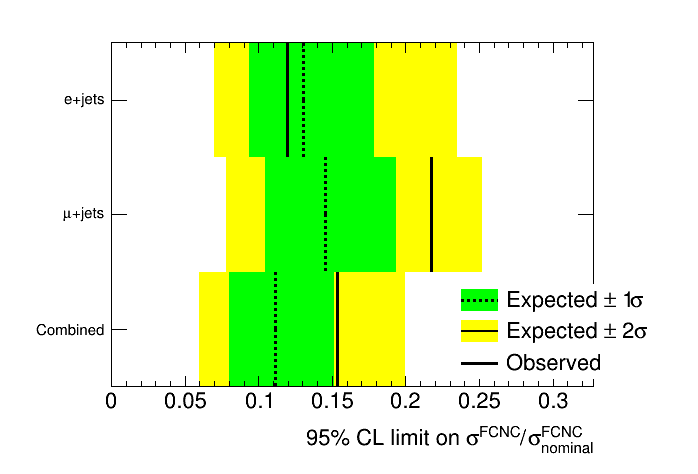
\includegraphics[width=0.5\columnwidth]{../ThesisImages/RegionPlots/FinalRegions/Systematics/LimitPlot.png}
	\caption{Limits on the signal strength $\mu$ for the alternative fit using $m_{q\gamma}$ in both regions.
	}
\end{figure}

\begin{table}[h!]
\begin{center}
{\renewcommand{\arraystretch}{1.2}
\begin{tabular}{ccccc}
\hhline{=====}
Channel  	&  Obs. Limit			&	Exp. Limit -$\sigma$	& Exp. Limit	& Exp. Limit +$\sigma$  \\  \hline 
e+jets	& $1.19\times10^{-4}$ 	& $0.94\times10^{-4}$	& $1.31\times10^{-4}$ & $1.78\times10^{-4}$	\\
$\mu$+jets	& $2.17\times10^{-4}$ 	& $1.04\times10^{-4}$	& $1.45\times10^{-4}$ & $1.93\times10^{-4}$	\\
Combined	& $1.54\times10^{-4}$ 	& $0.84\times10^{-4}$	& $1.12\times10^{-4}$ & $1.52\times10^{-4}$	\\
\hhline{=====}
\end{tabular}
\caption{Branching ratio limits for alternative fit using $m_{q\gamma}$ in both regions.}
}
\end{center}
\end{table}

\subsection{Validation Region Plots: Fit on  $m_{q\gamma}$ in $\mu$+jets Region}
\begin{figure}[]
\centering
\subfloat[]{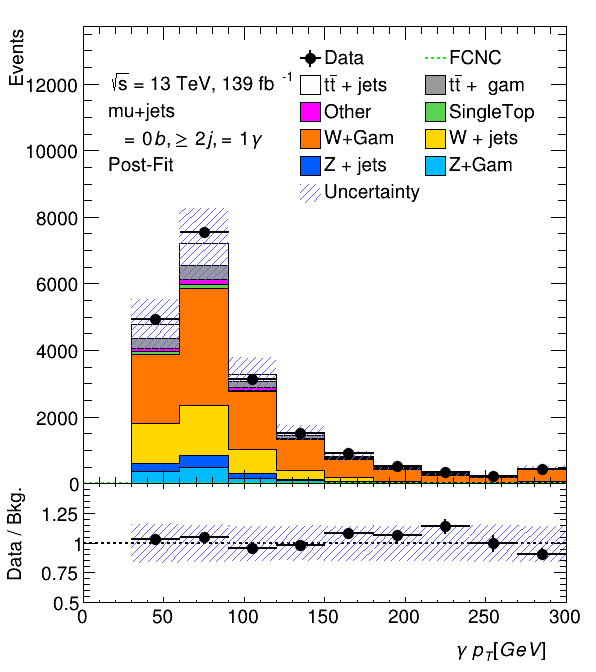
\includegraphics[width=.33\columnwidth]{../ThesisImages/RegionPlots/FinalRegions/Systematics/FCNC_All_mujets/Plots/VR1mu_ph_pt_postFit.png}}\hfil
\subfloat[]{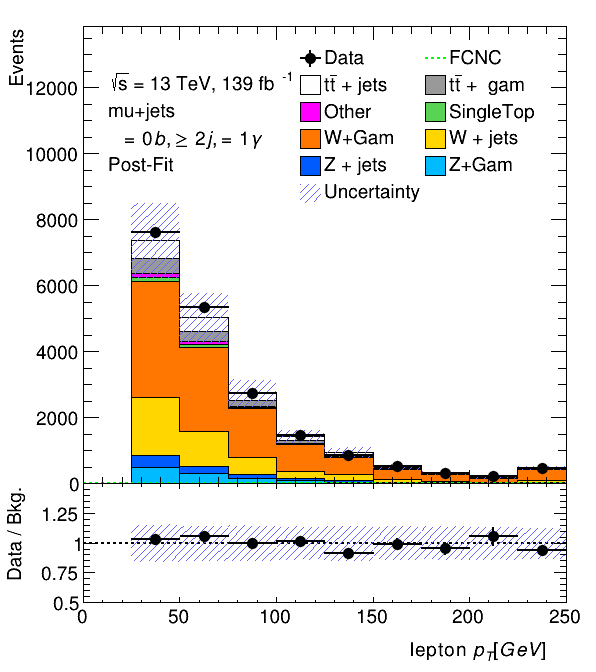
\includegraphics[width=.33\columnwidth]{../ThesisImages/RegionPlots/FinalRegions/Systematics/FCNC_All_mujets/Plots/VR1mu_lep_pt_postFit.png}}\hfil  
\subfloat[]{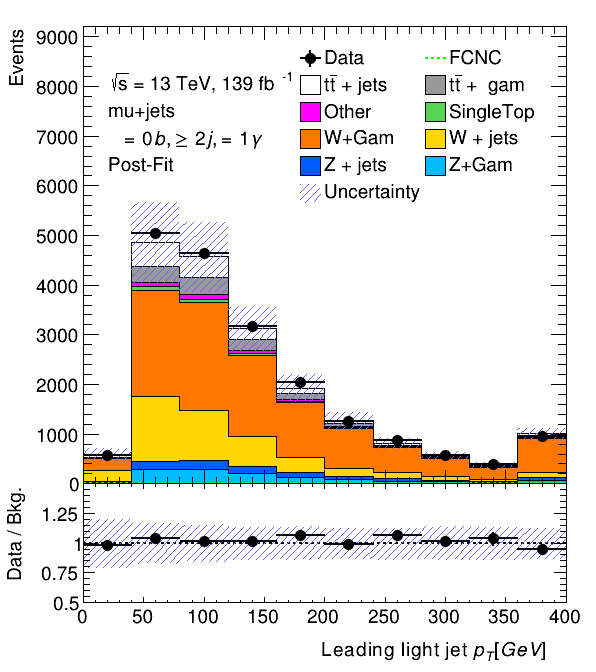
\includegraphics[width=.33\columnwidth]{../ThesisImages/RegionPlots/FinalRegions/Systematics/FCNC_All_mujets/Plots/VR1mu_jet0_pt_postFit.png}}
\vspace{-3.mm}
\subfloat[]{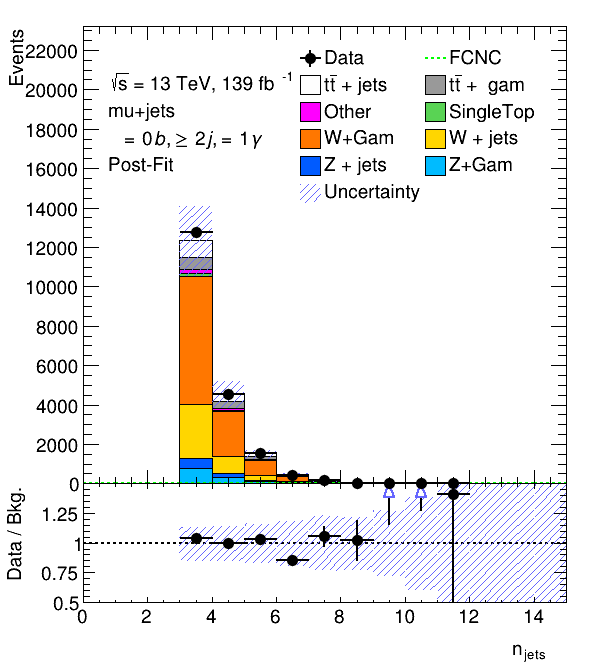
\includegraphics[width=.33\columnwidth]{../ThesisImages/RegionPlots/FinalRegions/Systematics/FCNC_All_mujets/Plots/VR1mu_njet_postFit.png}}\hfil
\subfloat[]{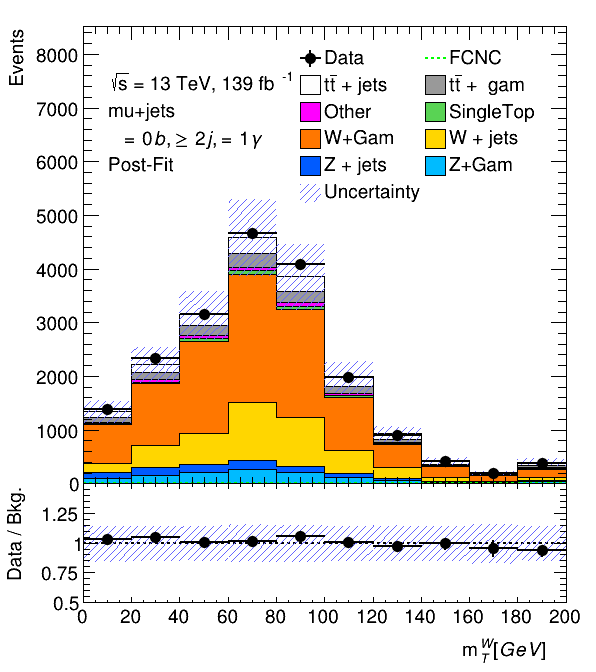
\includegraphics[width=.33\columnwidth]{../ThesisImages/RegionPlots/FinalRegions/Systematics/FCNC_All_mujets/Plots/VR1mu_MWT_postFit.png}}\hfil  
\subfloat[]{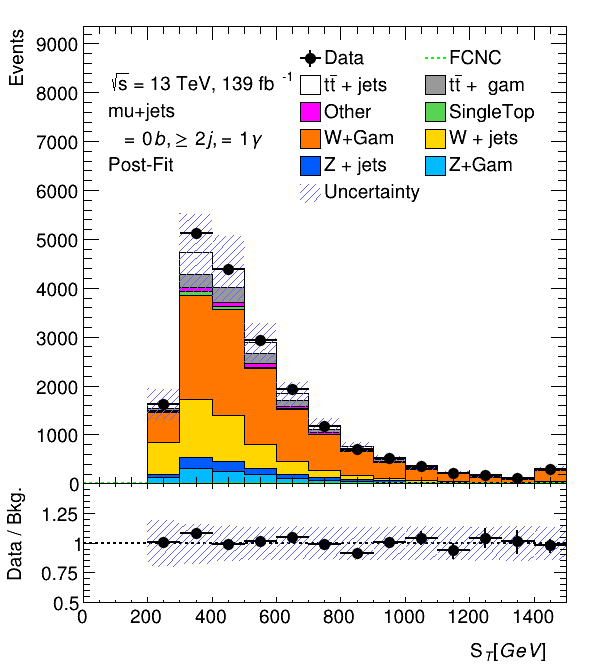
\includegraphics[width=.33\columnwidth]{../ThesisImages/RegionPlots/FinalRegions/Systematics/FCNC_All_mujets/Plots/VR1mu_ST_postFit.png}}
\caption{Post-fit distributions for Photon $p_T$ (a), lepton $p_T$ (b), leading light jet $p_T$ (c), $n_{jet}$ (d), $m_T^W$ (e), and $S_T$ (f) in the W+$\gamma$ validation region for the $\mu$+jets channel for alternative fit using  $m_{q\gamma}$ in both regions.}
\end{figure}


\begin{figure}[]
\centering
\subfloat[]{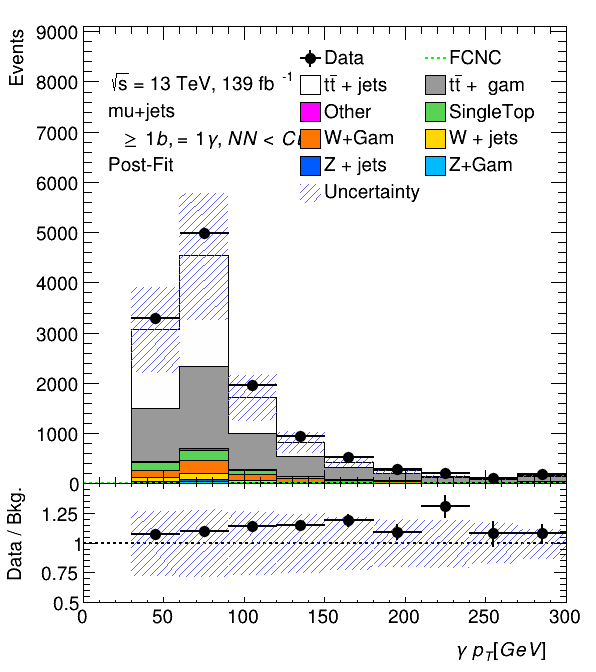
\includegraphics[width=.33\columnwidth]{../ThesisImages/RegionPlots/FinalRegions/Systematics/FCNC_All_mujets/Plots/VR2mu_ph_pt_postFit.png}}\hfil
\subfloat[]{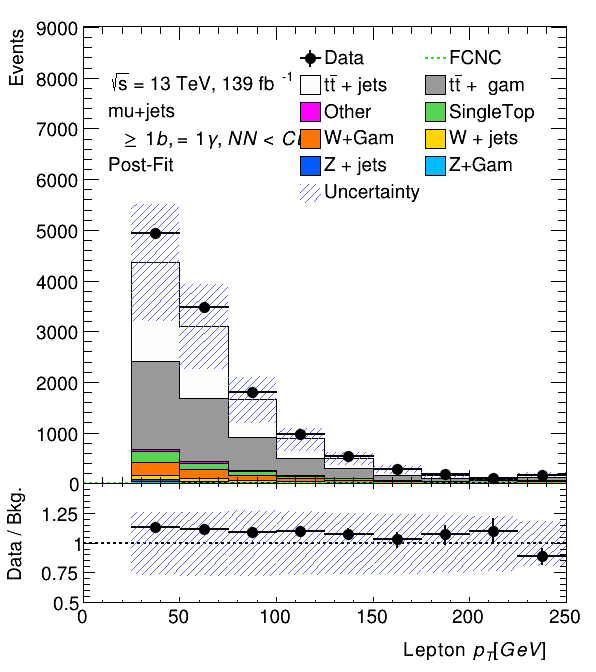
\includegraphics[width=.33\columnwidth]{../ThesisImages/RegionPlots/FinalRegions/Systematics/FCNC_All_mujets/Plots/VR2mu_lep_pt_postFit.png}}\hfil  
\subfloat[]{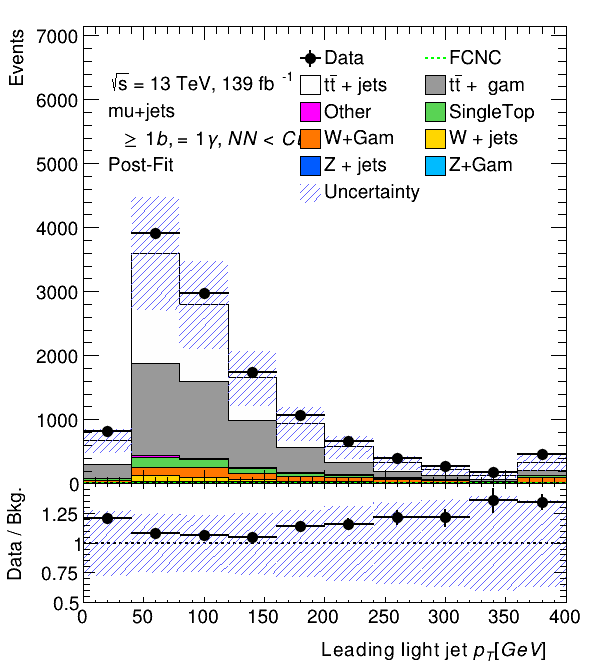
\includegraphics[width=.33\columnwidth]{../ThesisImages/RegionPlots/FinalRegions/Systematics/FCNC_All_mujets/Plots/VR2mu_jet0_pt_postFit.png}}
\vspace{-3.mm}
\subfloat[]{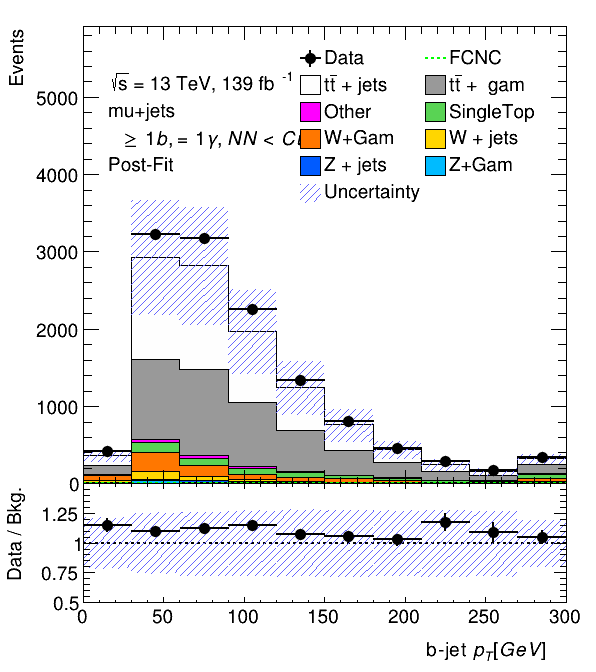
\includegraphics[width=.33\columnwidth]{../ThesisImages/RegionPlots/FinalRegions/Systematics/FCNC_All_mujets/Plots/VR2mu_bjet0_pt_postFit.png}}\hfil
\subfloat[]{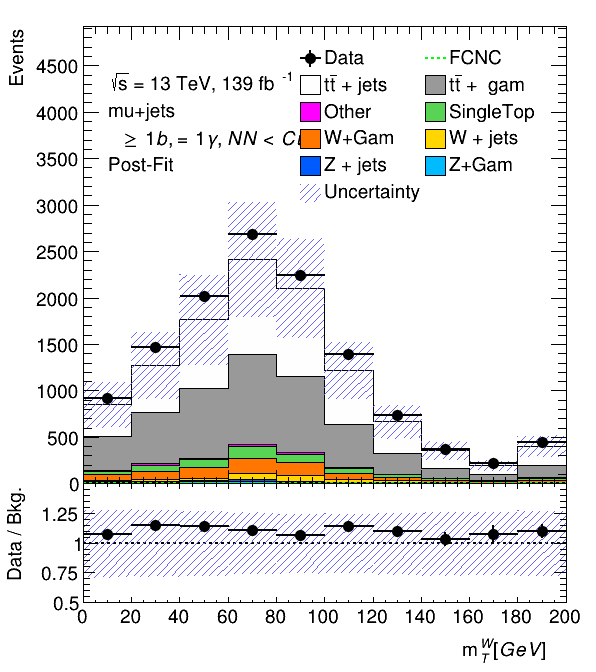
\includegraphics[width=.33\columnwidth]{../ThesisImages/RegionPlots/FinalRegions/Systematics/FCNC_All_mujets/Plots/VR2mu_MWT_postFit.png}}\hfil  
\subfloat[]{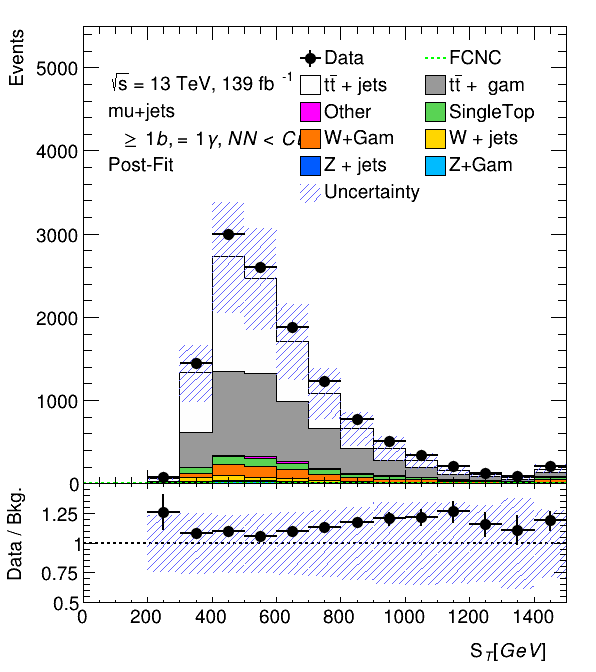
\includegraphics[width=.33\columnwidth]{../ThesisImages/RegionPlots/FinalRegions/Systematics/FCNC_All_mujets/Plots/VR2mu_ST_postFit.png}}
\caption{Post-fit distributions for Photon $p_T$ (a), lepton $p_T$ (b), leading light jet $p_T$ (c), leading b-jet $p_T$ (d),  $m_T^W$  (e), and $S_T$ (f) in the $t\bar{t}$+jets+$\gamma$ validation region for the $\mu$+jets channel for alternative fit using  $m_{q\gamma}$ in both regions.}
\end{figure}

%%%%%%%%%%%%%%%%%%%%%%%%

\section{Alternative Fit Method: Both Channels $\gamma$ $p_T$}
\label{sec:addfitel}

\begin{figure}[]
\centering
\subfloat[]{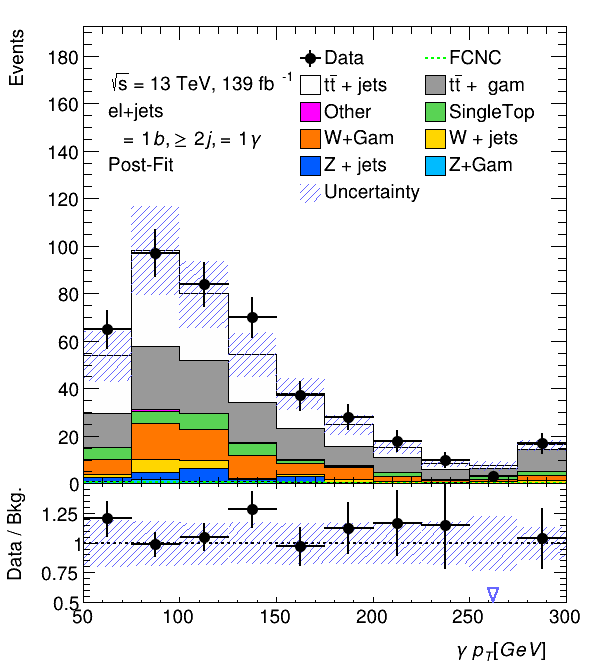
\includegraphics[width=.33\columnwidth]{../ThesisImages/RegionPlots/FinalRegions/Systematics/PhotonPT/FCNC_All_ejets/Plots/SR_ph_pt_postFit.png}}\hfil
\subfloat[]{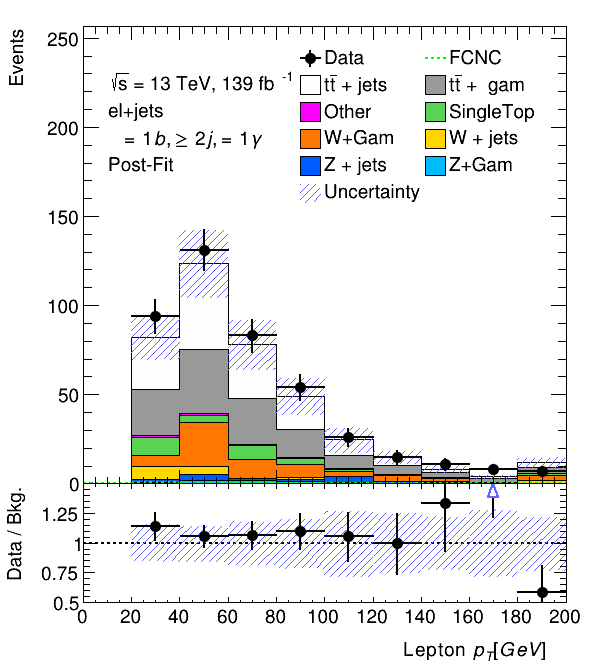
\includegraphics[width=.33\columnwidth]{../ThesisImages/RegionPlots/FinalRegions/Systematics/PhotonPT/FCNC_All_ejets/Plots/SR_lep_pt_postFit.png}}\hfil  
\subfloat[]{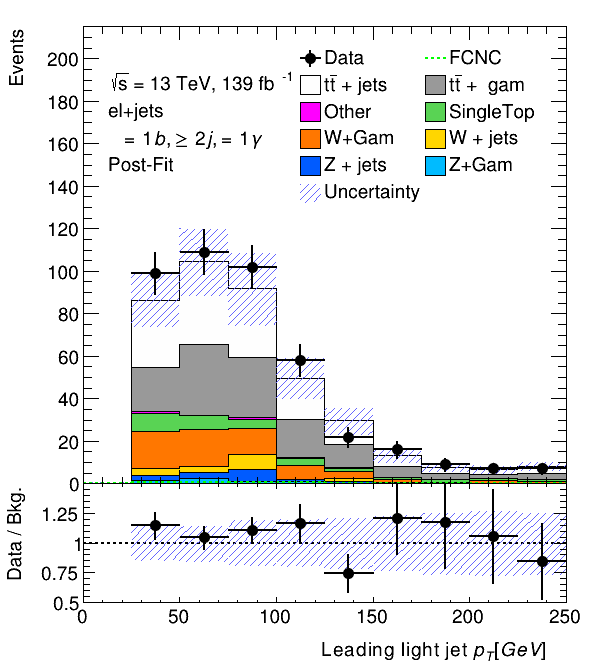
\includegraphics[width=.33\columnwidth]{../ThesisImages/RegionPlots/FinalRegions/Systematics/PhotonPT/FCNC_All_ejets/Plots/SR_jet0_pt_postFit.png}}
\vspace{-3.mm}
\subfloat[]{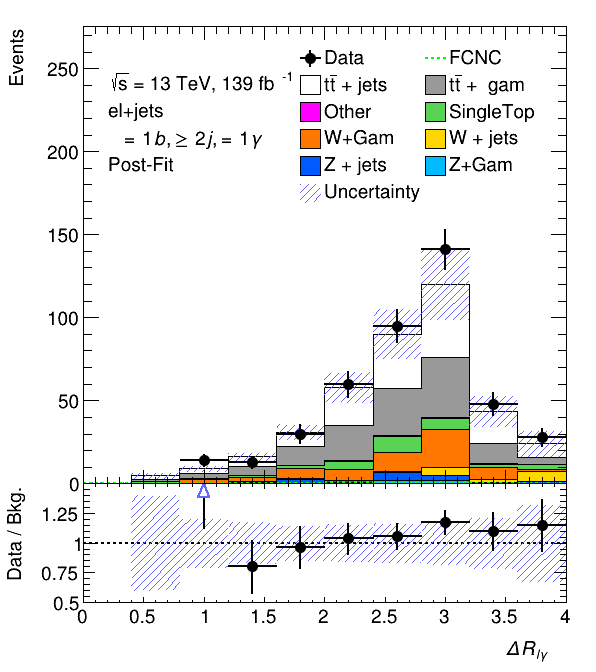
\includegraphics[width=.33\columnwidth]{../ThesisImages/RegionPlots/FinalRegions/Systematics/PhotonPT/FCNC_All_ejets/Plots/SR_drlph_postFit.png}}\hfil
\subfloat[]{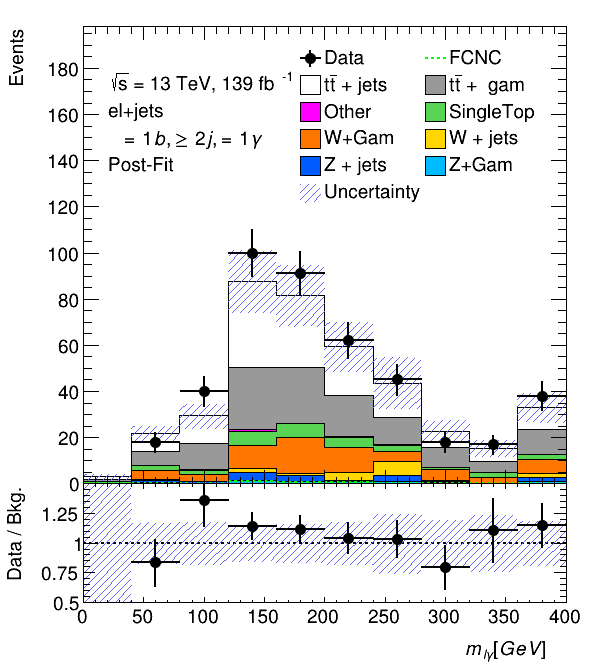
\includegraphics[width=.33\columnwidth]{../ThesisImages/RegionPlots/FinalRegions/Systematics/PhotonPT/FCNC_All_ejets/Plots/SR_m_lgam_postFit.png}}\hfil 
\subfloat[]{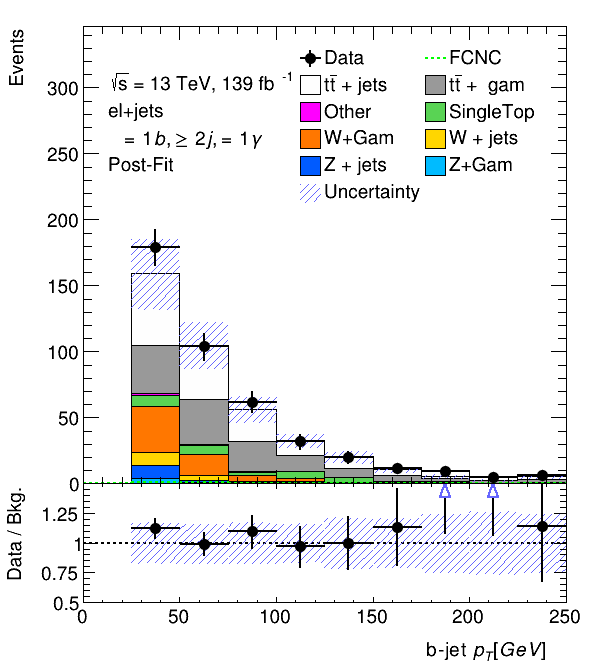
\includegraphics[width=.33\columnwidth]{../ThesisImages/RegionPlots/FinalRegions/Systematics/PhotonPT/FCNC_All_ejets/Plots/SR_bjet0_pt_postFit.png}}
\caption{Post-fit distributions for Photon $p_T$ (a), lepton $p_T$ (b), leading light jet $p_T$ (c), $\Delta R_{l\gamma}$ (d), $m_{l \gamma}$ (e), and b-jet $p_T$ (f) in the final signal region for the electron channel fitting on $\gamma$ $p_T$.}
\end{figure}


\begin{figure}[]
\centering
\subfloat[]{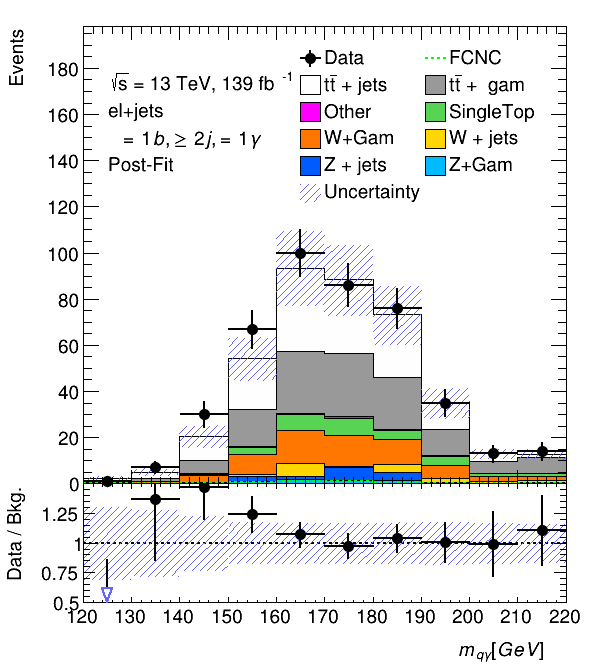
\includegraphics[width=.33\columnwidth]{../ThesisImages/RegionPlots/FinalRegions/Systematics/PhotonPT/FCNC_All_ejets/Plots/SR_mqph_postFit.png}}\hfil
\subfloat[]{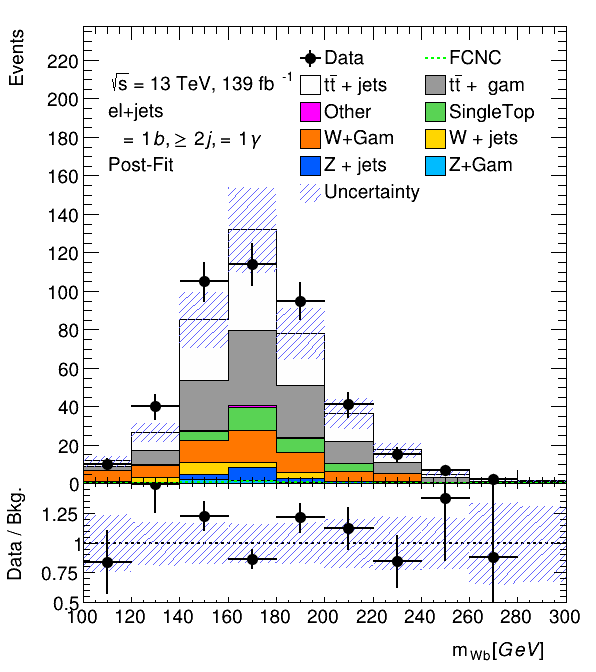
\includegraphics[width=.33\columnwidth]{../ThesisImages/RegionPlots/FinalRegions/Systematics/PhotonPT/FCNC_All_ejets/Plots/SR_SMtop_postFit.png}}\hfil  
\subfloat[]{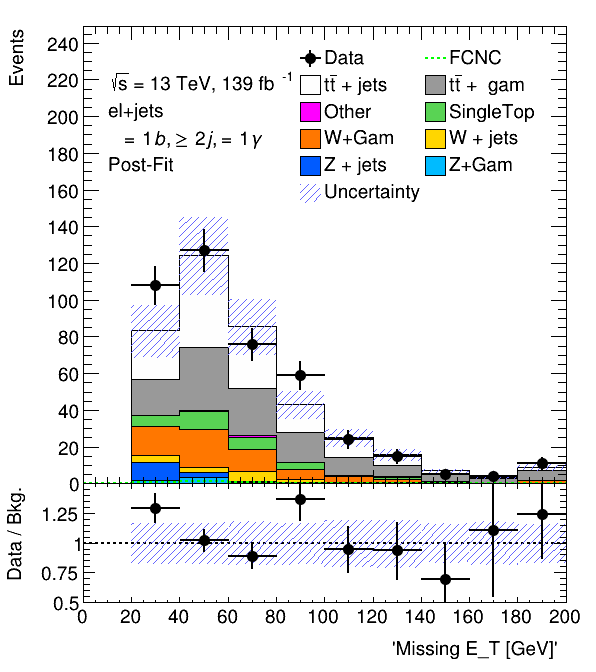
\includegraphics[width=.33\columnwidth]{../ThesisImages/RegionPlots/FinalRegions/Systematics/PhotonPT/FCNC_All_ejets/Plots/SR_met_postFit.png}}
\vspace{-3.mm}
\subfloat[]{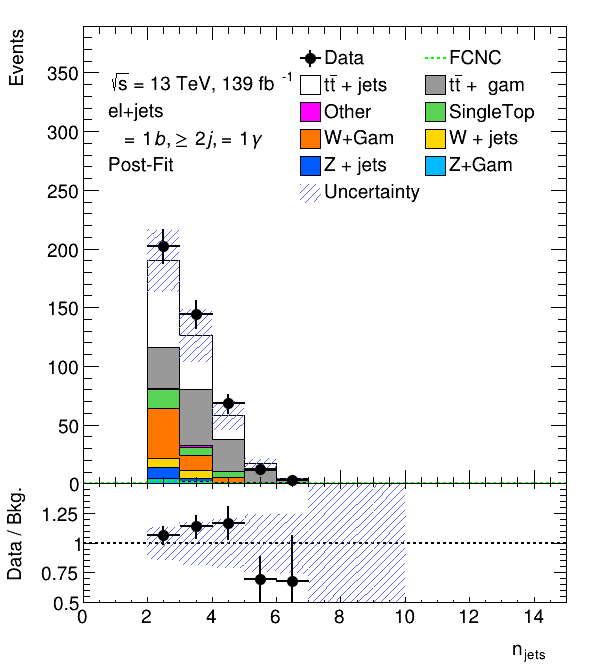
\includegraphics[width=.33\columnwidth]{../ThesisImages/RegionPlots/FinalRegions/Systematics/PhotonPT/FCNC_All_ejets/Plots/SR_njet_postFit.png}}\hfil
\subfloat[]{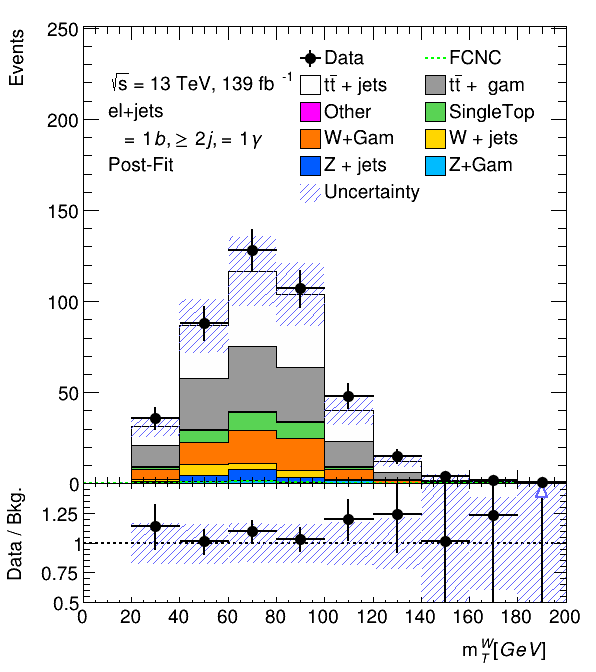
\includegraphics[width=.33\columnwidth]{../ThesisImages/RegionPlots/FinalRegions/Systematics/PhotonPT/FCNC_All_ejets/Plots/SR_MWT_postFit.png}}\hfil  
\subfloat[]{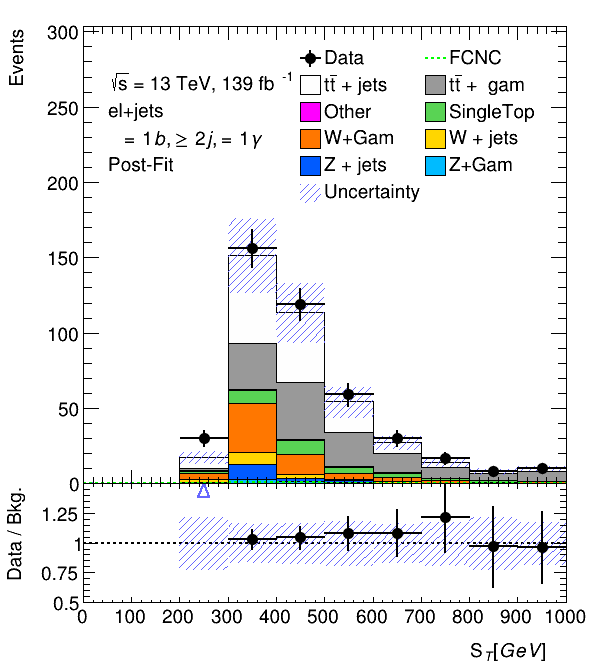
\includegraphics[width=.33\columnwidth]{../ThesisImages/RegionPlots/FinalRegions/Systematics/PhotonPT/FCNC_All_ejets/Plots/SR_ST_postFit.png}}
\caption{Post-fit distributions for FCNC top candidate mass (a), Standard Model top candidate mass (b), $\slashed{E}_T$ (c), $N_\text{jets}$ (d),  $m_T^W$ (e), and $S_T$ (f) in the final signal region for the electron channel fitting on $\gamma$ $p_T$.}
\end{figure}




\begin{figure}[ht!]
	\centering
	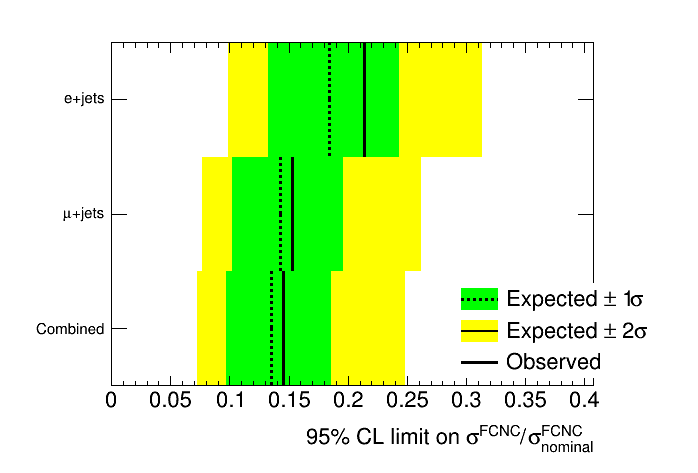
\includegraphics[width=0.5\columnwidth]{../ThesisImages/RegionPlots/FinalRegions/Systematics/PhotonPT/LimitPlot.png}
	\caption{Limits on the signal strength $\mu$ for the alternative fit using $\gamma$ $p_T$ in both regions.
	}
\end{figure}

\begin{table}[h!]
\begin{center}
{\renewcommand{\arraystretch}{1.2}
\begin{tabular}{ccccc}
\hhline{=====}
Channel  	&  Obs. Limit			&	Exp. Limit -$\sigma$	& Exp. Limit	& Exp. Limit +$\sigma$  \\  \hline 
e+jets	& $2.13\times10^{-4}$ 	& $1.31\times10^{-4}$	& $1.82\times10^{-4}$ & $2.42\times10^{-4}$	\\
$\mu$+jets	& $1.53\times10^{-4}$ 	& $1.03\times10^{-4}$	& $1.42\times10^{-4}$ & $1.96\times10^{-4}$	\\
Combined	& $1.47\times10^{-4}$ 	& $0.97\times10^{-4}$	& $1.34\times10^{-4}$ & $1.85\times10^{-4}$	\\
\hhline{=====}
\end{tabular}
\caption{Branching ratio limits for alternative fit using $\gamma$ $p_T$ in both regions.}
}
\end{center}
\end{table}


\subsection{Validation Region Plots: Fit on  $\gamma$ $p_T$ in e+jets Region}
\begin{figure}[]
\centering
\subfloat[]{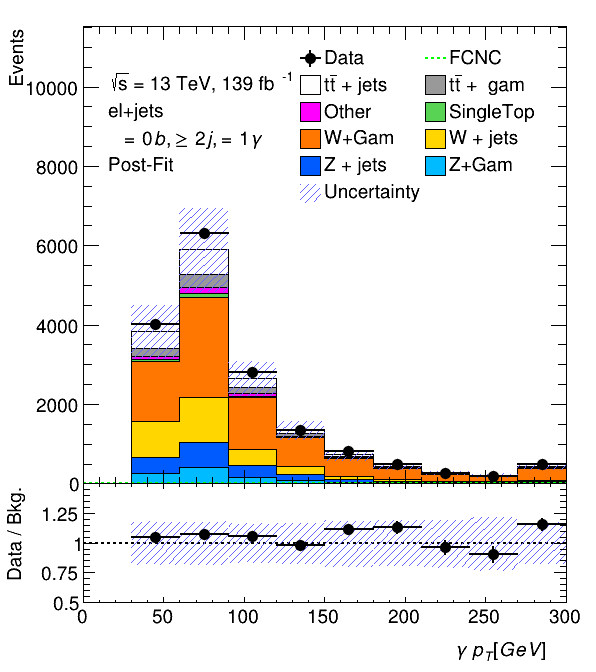
\includegraphics[width=.33\columnwidth]{../ThesisImages/RegionPlots/FinalRegions/Systematics/PhotonPT/FCNC_All_ejets/Plots/VR1_ph_pt_postFit.png}}\hfil
\subfloat[]{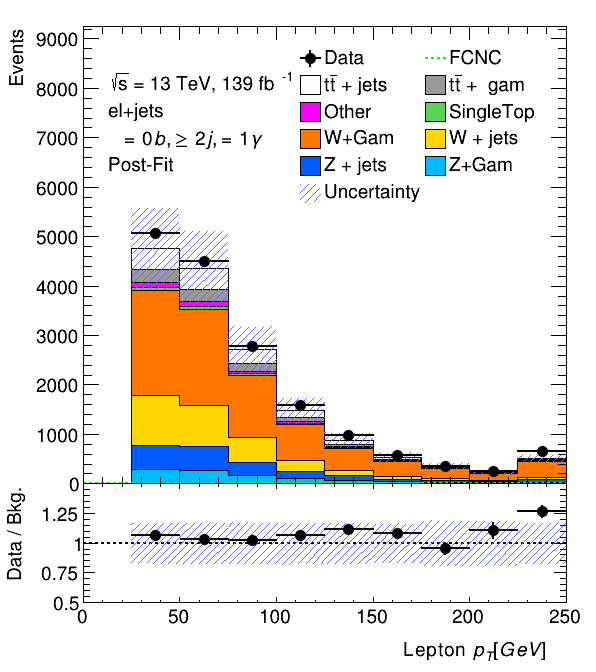
\includegraphics[width=.33\columnwidth]{../ThesisImages/RegionPlots/FinalRegions/Systematics/PhotonPT/FCNC_All_ejets/Plots/VR1_lep_pt_postFit.png}}\hfil  
\subfloat[]{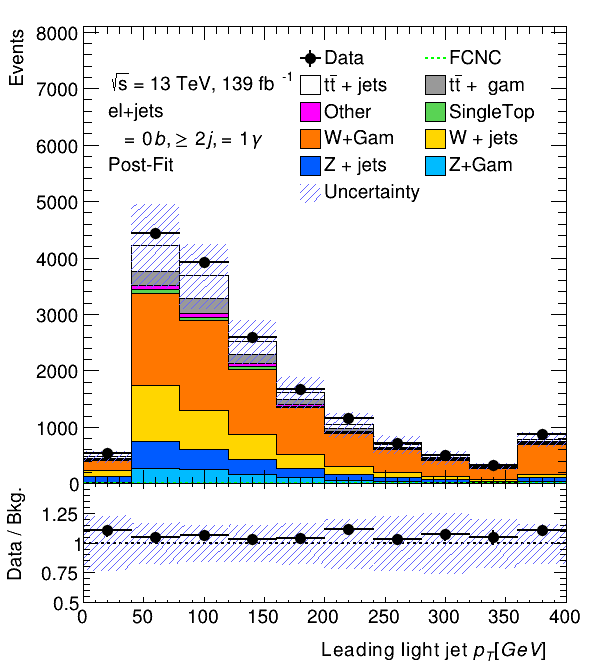
\includegraphics[width=.33\columnwidth]{../ThesisImages/RegionPlots/FinalRegions/Systematics/PhotonPT/FCNC_All_ejets/Plots/VR1_jet0_pt_postFit.png}}
\vspace{-3.mm}
\subfloat[]{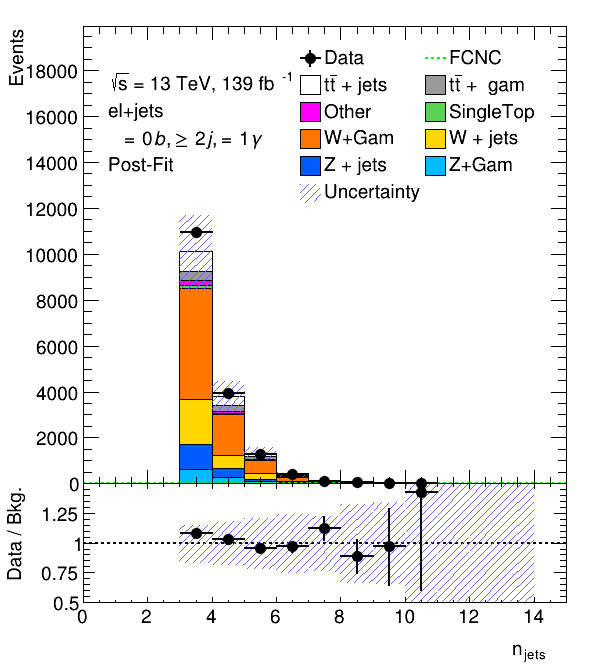
\includegraphics[width=.33\columnwidth]{../ThesisImages/RegionPlots/FinalRegions/Systematics/PhotonPT/FCNC_All_ejets/Plots/VR1_njet_postFit.png}}\hfil
\subfloat[]{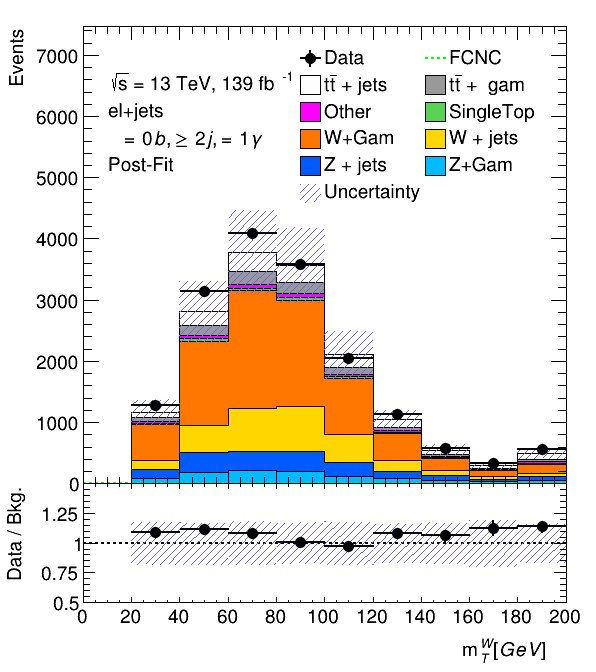
\includegraphics[width=.33\columnwidth]{../ThesisImages/RegionPlots/FinalRegions/Systematics/PhotonPT/FCNC_All_ejets/Plots/VR1_MWT_postFit.png}}\hfil  
\subfloat[]{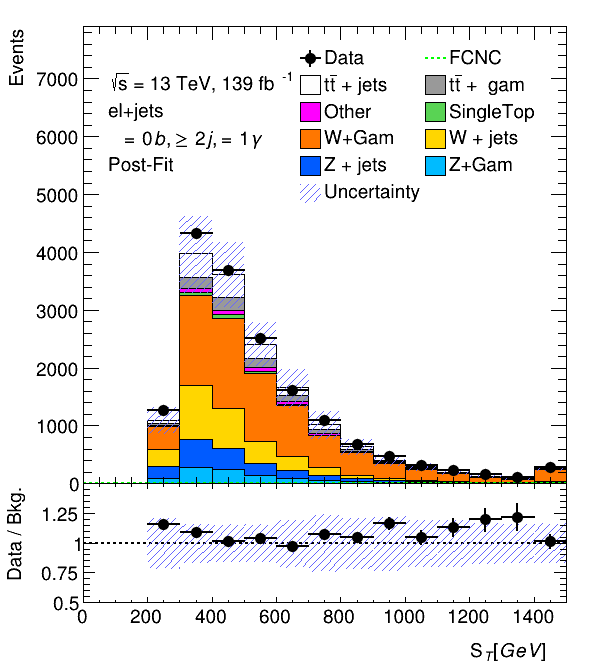
\includegraphics[width=.33\columnwidth]{../ThesisImages/RegionPlots/FinalRegions/Systematics/PhotonPT/FCNC_All_ejets/Plots/VR1_ST_postFit.png}}
\caption{Post-fit distributions for Photon $p_T$ (a), lepton $p_T$ (b), leading light jet $p_T$ (c), $n_{jet}$ (d), $m_T^W$ (e), and $S_T$ (f) in the W+$\gamma$ validation region for the e+jets channel for alternative fit using  $\gamma$ $p_T$ in both regions. }
\end{figure}


%\section{e+jets fit, $t\bar{t}$+$\gamma$ Validation Region}
\begin{figure}[]
\centering
\subfloat[]{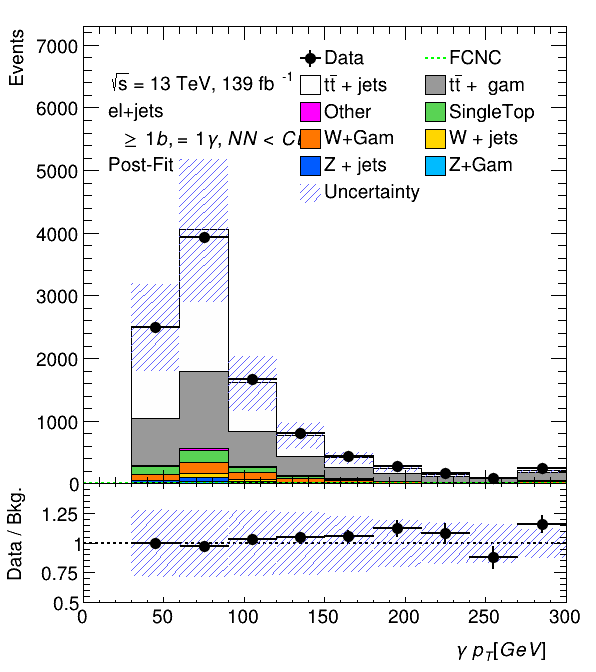
\includegraphics[width=.33\columnwidth]{../ThesisImages/RegionPlots/FinalRegions/Systematics/PhotonPT/FCNC_All_ejets/Plots/VR2_ph_pt_postFit.png}}\hfil
\subfloat[]{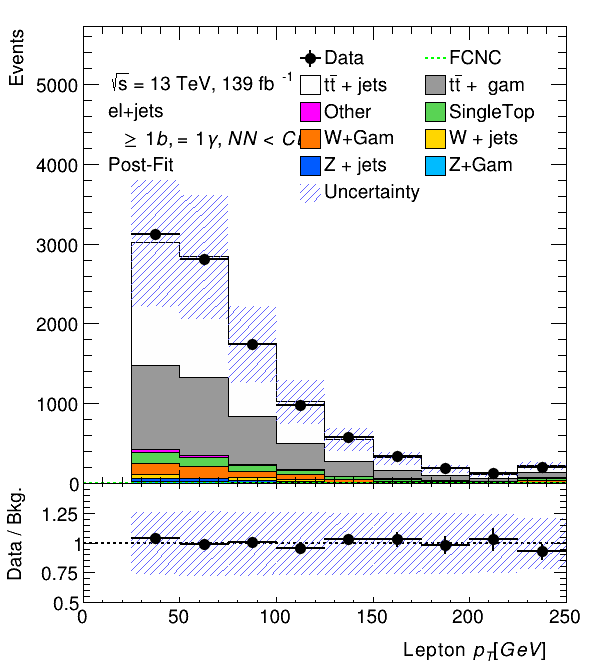
\includegraphics[width=.33\columnwidth]{../ThesisImages/RegionPlots/FinalRegions/Systematics/PhotonPT/FCNC_All_ejets/Plots/VR2_lep_pt_postFit.png}}\hfil  
\subfloat[]{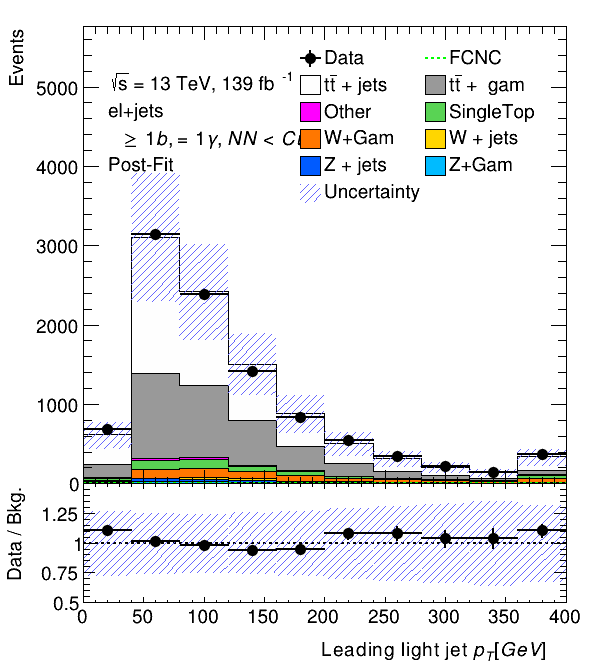
\includegraphics[width=.33\columnwidth]{../ThesisImages/RegionPlots/FinalRegions/Systematics/PhotonPT/FCNC_All_ejets/Plots/VR2_jet0_pt_postFit.png}}
\vspace{-3.mm}
\subfloat[]{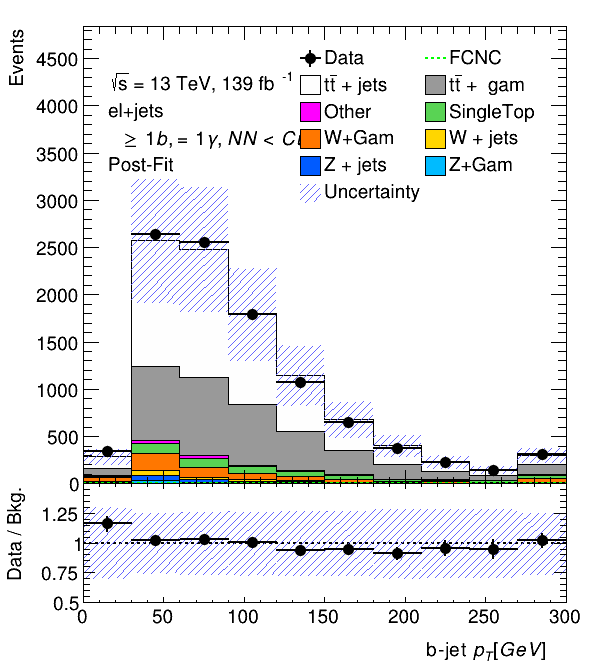
\includegraphics[width=.33\columnwidth]{../ThesisImages/RegionPlots/FinalRegions/Systematics/PhotonPT/FCNC_All_ejets/Plots/VR2_bjet0_pt_postFit.png}}\hfil
\subfloat[]{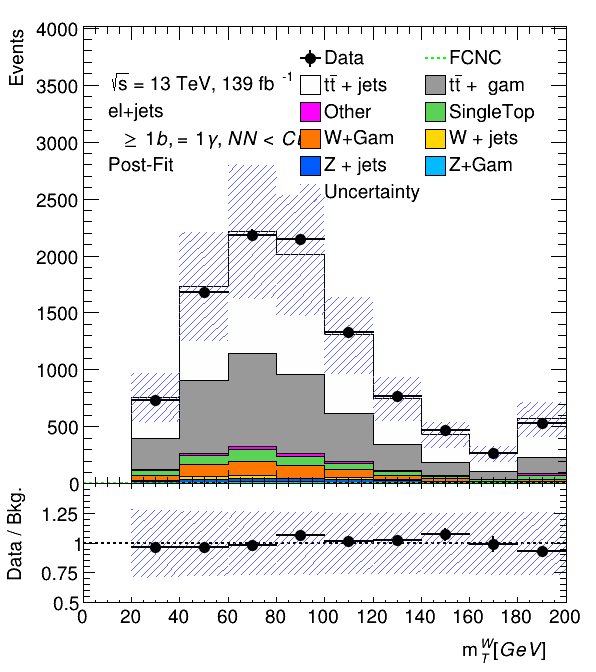
\includegraphics[width=.33\columnwidth]{../ThesisImages/RegionPlots/FinalRegions/Systematics/PhotonPT/FCNC_All_ejets/Plots/VR2_MWT_postFit.png}}\hfil  
\subfloat[]{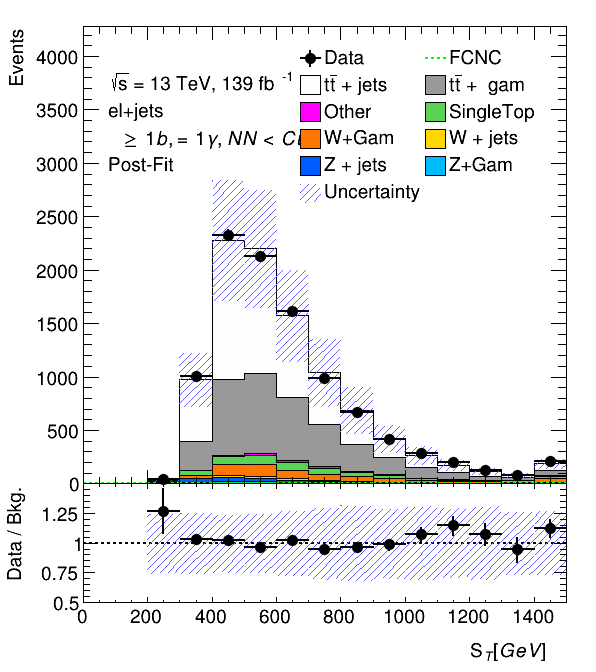
\includegraphics[width=.33\columnwidth]{../ThesisImages/RegionPlots/FinalRegions/Systematics/PhotonPT/FCNC_All_ejets/Plots/VR2_ST_postFit.png}}
\caption{Post-fit distributions for Photon $p_T$ (a), lepton $p_T$ (b), leading light jet $p_T$ (c), leading b-jet $p_T$ (d),  $m_T^W$  (e), and $S_T$ (f) in the $t\bar{t}$+jets+$\gamma$ validation region for the  e+jets channel for alternative fit using  $\gamma$ $p_T$ in both regions. }
\end{figure}



















